\documentclass[tikz,border=20pt]{standalone}
\usetikzlibrary{calc,arrows.meta,shapes.geometric}
\usepackage{amsmath,amssymb}

\definecolor{steelcolor}{HTML}{475569}
\definecolor{darksteel}{HTML}{1E293B}
\definecolor{linkwhite}{HTML}{F1F5F9}
\definecolor{jointorange}{HTML}{EA580C}

\begin{document}
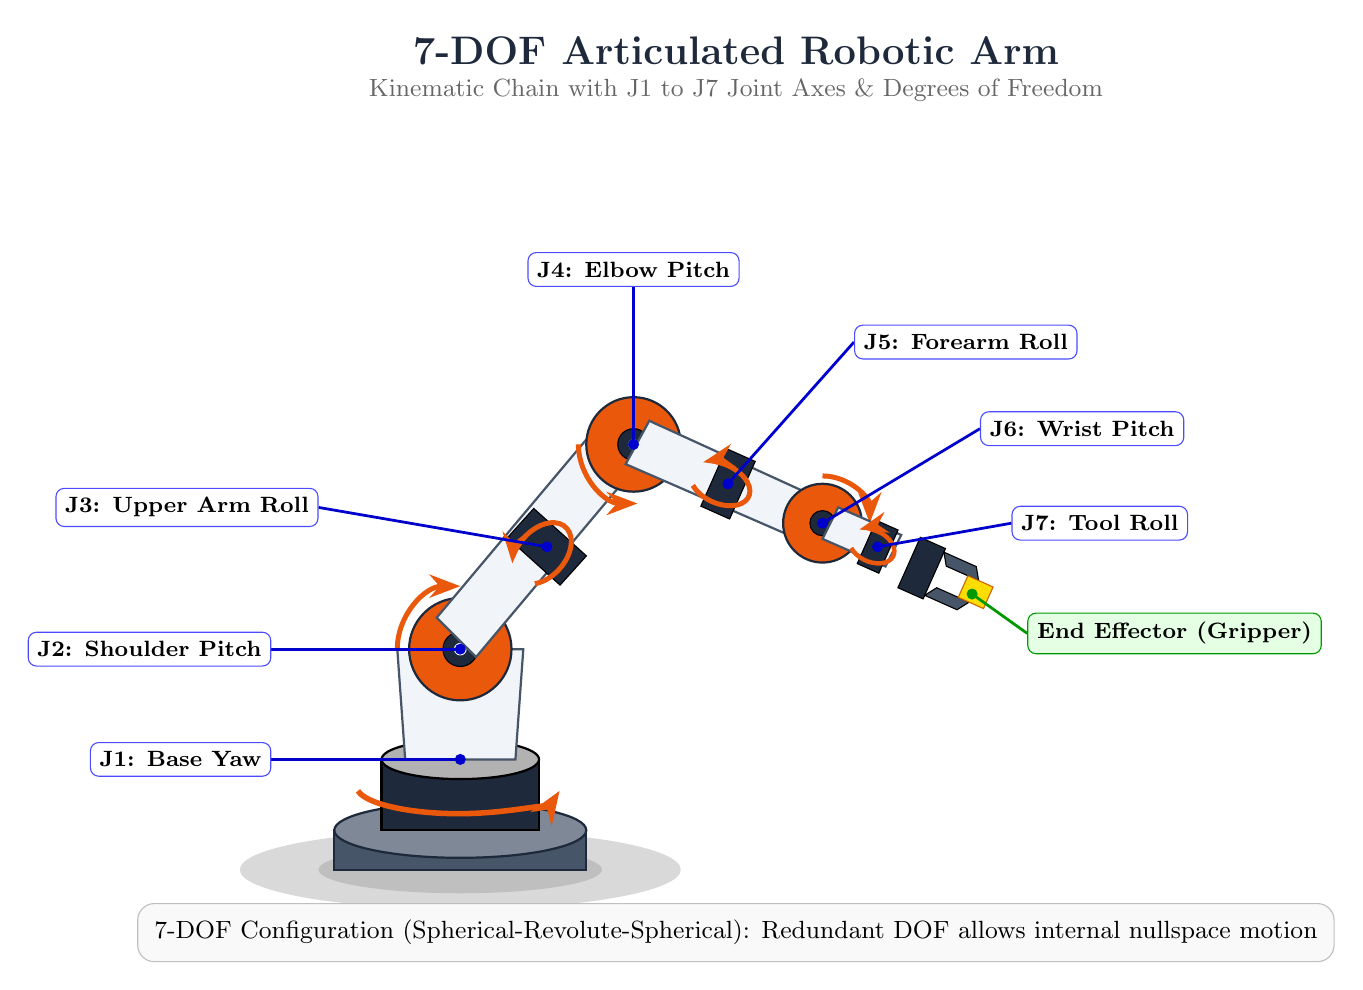
\begin{tikzpicture}[x=1cm, y=1cm, >=Stealth]

  % Title
  \node[font=\bfseries\Large, text=darksteel] at (3.5, 6.2) {7-DOF Articulated Robotic Arm};
  \node[font=\small, text=gray!80!black] at (3.5, 5.7) {Kinematic Chain with J1 to J7 Joint Axes \& Degrees of Freedom};

  % Floor & Pedestal Shadow
  \fill[gray!30] (0, -4.2) ellipse (2.8 and 0.5);
  \fill[gray!50] (0, -4.2) ellipse (1.8 and 0.3);

  % 1. BASE FLANGE (Stationary)
  \filldraw[fill=steelcolor, draw=darksteel, thick] (-1.6, -4.2) rectangle (1.6, -3.7);
  \filldraw[fill=steelcolor!70, draw=darksteel, thick] (0, -3.7) ellipse (1.6 and 0.35);

  % 2. J1 TURNTABLE (Base Yaw)
  \filldraw[fill=darksteel, draw=black, thick] (-1.0, -3.7) rectangle (1.0, -2.8);
  \filldraw[fill=gray!60, draw=black, thick] (0, -2.8) ellipse (1.0 and 0.25);
  % J1 Rotation Arrow
  \draw[->, line width=2pt, color=jointorange] (-1.3, -3.2) arc (190:350:1.3 and 0.35);

  % 3. LINK 1 & J2 (Shoulder Pitch: at 0, -1.4)
  \filldraw[fill=linkwhite, draw=steelcolor, thick] (-0.7, -2.8) -- (-0.8, -1.4) -- (0.8, -1.4) -- (0.7, -2.8) -- cycle;
  % J2 Joint Drum
  \filldraw[fill=jointorange, draw=darksteel, thick] (0, -1.4) circle (0.65);
  \filldraw[fill=darksteel, draw=black] (0, -1.4) circle (0.22);
  \fill[white] (0, -1.4) circle (0.08);
  % J2 Rotation Arrow
  \draw[->, line width=1.8pt, color=jointorange] (-0.8, -1.4) arc (180:90:0.8);

  % 4. LINK 2 & J3 (Upper Arm Roll: extending from (0, -1.4) to (2.2, 1.2))
  \filldraw[fill=linkwhite, draw=steelcolor, thick]
    (-0.3, -1.0) -- (1.8, 1.5) -- (2.3, 1.0) -- (0.2, -1.5) -- cycle;
  % J3 Roll Joint Collar (at (1.1, -0.1))
  \begin{scope}[shift={(1.1, -0.1)}, rotate=48]
    \filldraw[fill=darksteel, draw=black] (-0.25, -0.45) rectangle (0.25, 0.45);
    \draw[->, line width=1.8pt, color=jointorange] (-0.45, -0.2) arc (-140:140:0.45 and 0.3);
  \end{scope}

  % 5. J4 (Elbow Pitch: at (2.2, 1.2))
  \filldraw[fill=jointorange, draw=darksteel, thick] (2.2, 1.2) circle (0.6);
  \filldraw[fill=darksteel, draw=black] (2.2, 1.2) circle (0.2);
  \fill[white] (2.2, 1.2) circle (0.07);
  % J4 Rotation Arrow
  \draw[->, line width=1.8pt, color=jointorange] (1.5, 1.2) arc (180:270:0.75);

  % 6. LINK 3 & J5 (Forearm Roll: extending from (2.2, 1.2) down-right to (4.6, 0.2))
  \filldraw[fill=linkwhite, draw=steelcolor, thick]
    (2.4, 1.5) -- (4.7, 0.45) -- (4.4, -0.05) -- (2.1, 0.95) -- cycle;
  % J5 Roll Joint Collar (at (3.4, 0.7))
  \begin{scope}[shift={(3.4, 0.7)}, rotate=-24]
    \filldraw[fill=darksteel, draw=black] (-0.2, -0.4) rectangle (0.2, 0.4);
    \draw[->, line width=1.8pt, color=jointorange] (-0.4, -0.2) arc (-140:140:0.4 and 0.25);
  \end{scope}

  % 7. J6 (Wrist Pitch: at (4.6, 0.2))
  \filldraw[fill=jointorange, draw=darksteel, thick] (4.6, 0.2) circle (0.5);
  \filldraw[fill=darksteel, draw=black] (4.6, 0.2) circle (0.16);
  \fill[white] (4.6, 0.2) circle (0.05);
  % J6 Rotation Arrow
  \draw[->, line width=1.8pt, color=jointorange] (4.6, 0.8) arc (90:0:0.6);

  % 8. LINK 4 & J7 (Tool Flange Roll: at (5.4, -0.15))
  \filldraw[fill=linkwhite, draw=steelcolor, thick]
    (4.8, 0.4) -- (5.6, 0.05) -- (5.4, -0.35) -- (4.6, -0.0) -- cycle;
  % J7 Roll Collar
  \begin{scope}[shift={(5.3, -0.1)}, rotate=-24]
    \filldraw[fill=darksteel, draw=black] (-0.15, -0.3) rectangle (0.15, 0.3);
    \draw[->, line width=1.6pt, color=jointorange] (-0.3, -0.15) arc (-140:140:0.3 and 0.2);
  \end{scope}

  % 9. END EFFECTOR (Gripper & Workpiece)
  \begin{scope}[shift={(5.7, -0.3)}, rotate=-24]
    % Gripper Base
    \filldraw[fill=darksteel, draw=black] (0, -0.35) rectangle (0.35, 0.35);
    % Fingers
    \filldraw[fill=steelcolor, draw=black] (0.35, -0.3) -- (0.8, -0.3) -- (0.9, -0.15) -- (0.45, -0.15) -- cycle;
    \filldraw[fill=steelcolor, draw=black] (0.35, 0.3) -- (0.8, 0.3) -- (0.9, 0.15) -- (0.45, 0.15) -- cycle;
    % Gripped object
    \filldraw[fill=yellow!80!orange, draw=orange!80!black] (0.75, -0.15) rectangle (1.1, 0.15);
  \end{scope}

  % CALLOUT LABELS (J1 to J7)
  % J1
  \draw[blue!80!black, line width=1pt] (0, -2.8) -- (-2.4, -2.8);
  \fill[blue!80!black] (0, -2.8) circle (2pt);
  \node[draw=blue!70, fill=white, rounded corners=3pt, font=\bfseries\footnotesize, left] at (-2.4, -2.8) {J1: Base Yaw};

  % J2
  \draw[blue!80!black, line width=1pt] (0, -1.4) -- (-2.4, -1.4);
  \fill[blue!80!black] (0, -1.4) circle (2pt);
  \node[draw=blue!70, fill=white, rounded corners=3pt, font=\bfseries\footnotesize, left] at (-2.4, -1.4) {J2: Shoulder Pitch};

  % J3
  \draw[blue!80!black, line width=1pt] (1.1, -0.1) -- (-1.8, 0.4);
  \fill[blue!80!black] (1.1, -0.1) circle (2pt);
  \node[draw=blue!70, fill=white, rounded corners=3pt, font=\bfseries\footnotesize, left] at (-1.8, 0.4) {J3: Upper Arm Roll};

  % J4
  \draw[blue!80!black, line width=1pt] (2.2, 1.2) -- (2.2, 3.2);
  \fill[blue!80!black] (2.2, 1.2) circle (2pt);
  \node[draw=blue!70, fill=white, rounded corners=3pt, font=\bfseries\footnotesize, above] at (2.2, 3.2) {J4: Elbow Pitch};

  % J5
  \draw[blue!80!black, line width=1pt] (3.4, 0.7) -- (5.0, 2.5);
  \fill[blue!80!black] (3.4, 0.7) circle (2pt);
  \node[draw=blue!70, fill=white, rounded corners=3pt, font=\bfseries\footnotesize, right] at (5.0, 2.5) {J5: Forearm Roll};

  % J6
  \draw[blue!80!black, line width=1pt] (4.6, 0.2) -- (6.6, 1.4);
  \fill[blue!80!black] (4.6, 0.2) circle (2pt);
  \node[draw=blue!70, fill=white, rounded corners=3pt, font=\bfseries\footnotesize, right] at (6.6, 1.4) {J6: Wrist Pitch};

  % J7
  \draw[blue!80!black, line width=1pt] (5.3, -0.1) -- (7.0, 0.2);
  \fill[blue!80!black] (5.3, -0.1) circle (2pt);
  \node[draw=blue!70, fill=white, rounded corners=3pt, font=\bfseries\footnotesize, right] at (7.0, 0.2) {J7: Tool Roll};

  % End Effector Callout
  \draw[green!60!black, line width=1pt] (6.5, -0.7) -- (7.2, -1.2);
  \fill[green!60!black] (6.5, -0.7) circle (2pt);
  \node[draw=green!60!black, fill=green!10, rounded corners=3pt, font=\bfseries\footnotesize, right] at (7.2, -1.2) {End Effector (Gripper)};

  % Redundancy note
  \node[draw=gray!50, fill=gray!5, rounded corners=6pt, font=\small, inner sep=6pt] at (3.5, -5.0) {
    7-DOF Configuration (Spherical-Revolute-Spherical): Redundant DOF allows internal nullspace motion
  };

\end{tikzpicture}
\end{document}
